% Chapter 1

\chapter{Introducción general} % Main chapter title

\label{Chapter1} % For referencing the chapter elsewhere, use \ref{Chapter1} 
\label{IntroGeneral}

En este capítulo se presenta una introducción general al trabajo realizado. Se describe el problema que el \textit{Rhynchophorus Ferrugineus} (picudo rojo) presenta en las palmeras de la ciudad de Montevideo, el estado del arte en cuanto a trabajos similares y los objetivos planteados por la Intendencia de Montevideo (IM) y por el equipo de trabajo.

%--------------------------------------------------------------------------------------------------------------------------------------------------------------------------------

% Define some commands to keep the formatting separated from the content 
\newcommand{\keyword}[1]{\textbf{#1}}
\newcommand{\tabhead}[1]{\textbf{#1}}
\newcommand{\code}[1]{\texttt{#1}}
\newcommand{\file}[1]{\texttt{\bfseries#1}}
\newcommand{\option}[1]{\texttt{\itshape#1}}
\newcommand{\grados}{$^{\circ}$}
\newcommand{\comment}[1]{}

%--------------------------------------------------------------------------------------------------------------------------------------------------------------------------------
\section{Descripción del problema}
\label{sec:descProblema}

El picudo rojo, que puede observarse en la figura \ref{fig:picudo-rojo}, es un insecto que afecta a las palmeras, especialmente a la \textit{Phoenix Canariensis}, que es la especie más común en Montevideo. Este insecto ha causado un daño significativo en la flora de la ciudad, lo que ha llevado a la IM a enfocarse en su control y erradicación.

\begin{figure}[htpb]
  \centering
  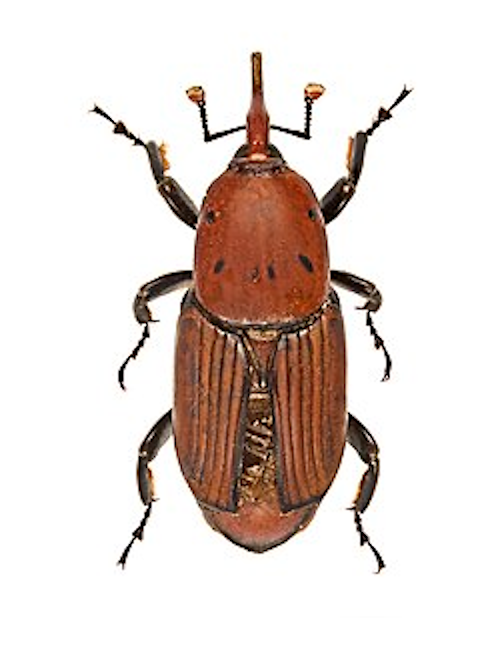
\includegraphics[scale=1]{./Figures/picudo-rojo.png}
  \caption{Picudo rojo \protect\footnotemark.}
  \label{fig:picudo-rojo}
\end{figure}

\footnotetext{Imagen tomada de \url{https://es.wikipedia.org/wiki/Rhynchophorus_ferrugineus}}

Este escarabajo supone una amenaza grave para las palmeras infectadas ya que las larvas de este insecto se alimentan del tejido interno de la planta, causando su colapso estructural en un período de meses (dada la gran cantidad de larvas que genera cada hembra \citep{anticimex_picudo_nodate}), como puede verse en la figura \ref{fig:palmera-infectada}. Esta amenaza aumenta según la época del año, puesto que el insecto tiene diferentes tasas de dispersión y reproducción dependiendo de la temperatura y la humedad. Existen varios tipos de picudos \citep{poplin_palm_2014}, algunos autóctonos y otros introducidos.

La plaga del picudo rojo llegó a Uruguay en 2022 \citep{mgap_informacion_nodate}, y se esparció rápidamente por la ciudad de Montevideo. De las 25 000 palmeras que forman una parte esencial de la ciudad, muchas ya han sucumbido a la plaga, donde se estima que para el año 2030 el ecosistema se verá ampliamente afectado \citep{arcos_picudo_2024} si no se toman medidas de control adecuadas. Últimamente también se ha esparcido por el interior del país, como puede observarse en la figura \ref{fig:palmeras-ruta5}, perteneciente a la ruta 5 de Uruguay, donde se han encontrado palmeras muertas por la plaga.

\begin{figure}[htpb]
  \centering
  \begin{subfigure}[b]{0.49\textwidth}
    \centering
    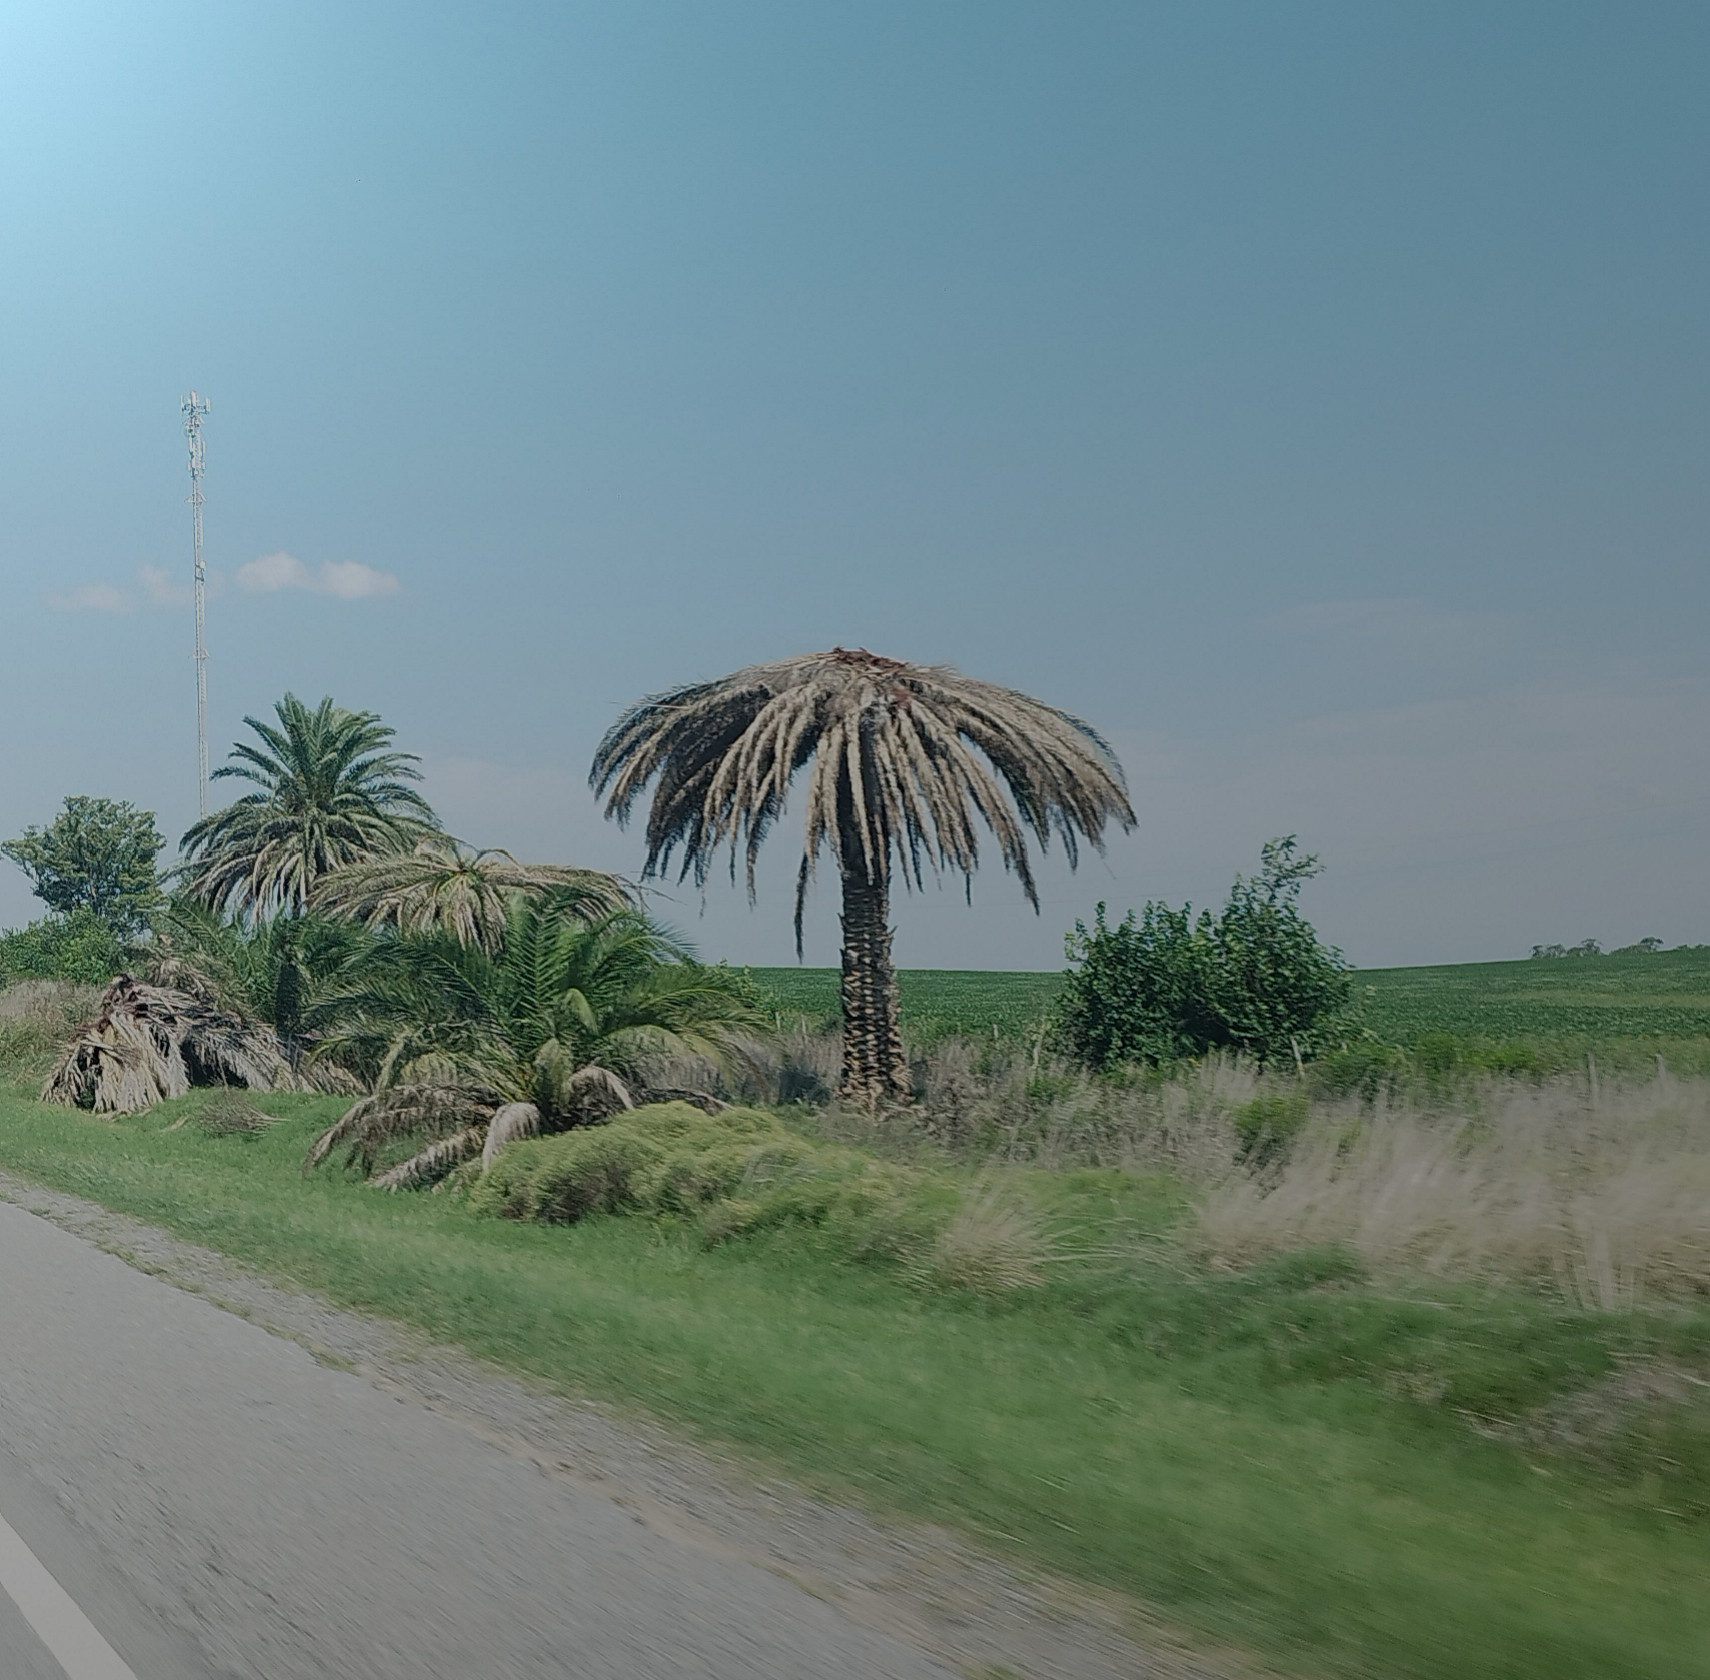
\includegraphics[width=\textwidth]{./Figures/palmera-infectada.jpg}
    \caption{Palmera infectada por el picudo rojo.}
    \label{fig:palmera-infectada}
  \end{subfigure}
  \hfill
  \begin{subfigure}[b]{0.49\textwidth}
    \centering
    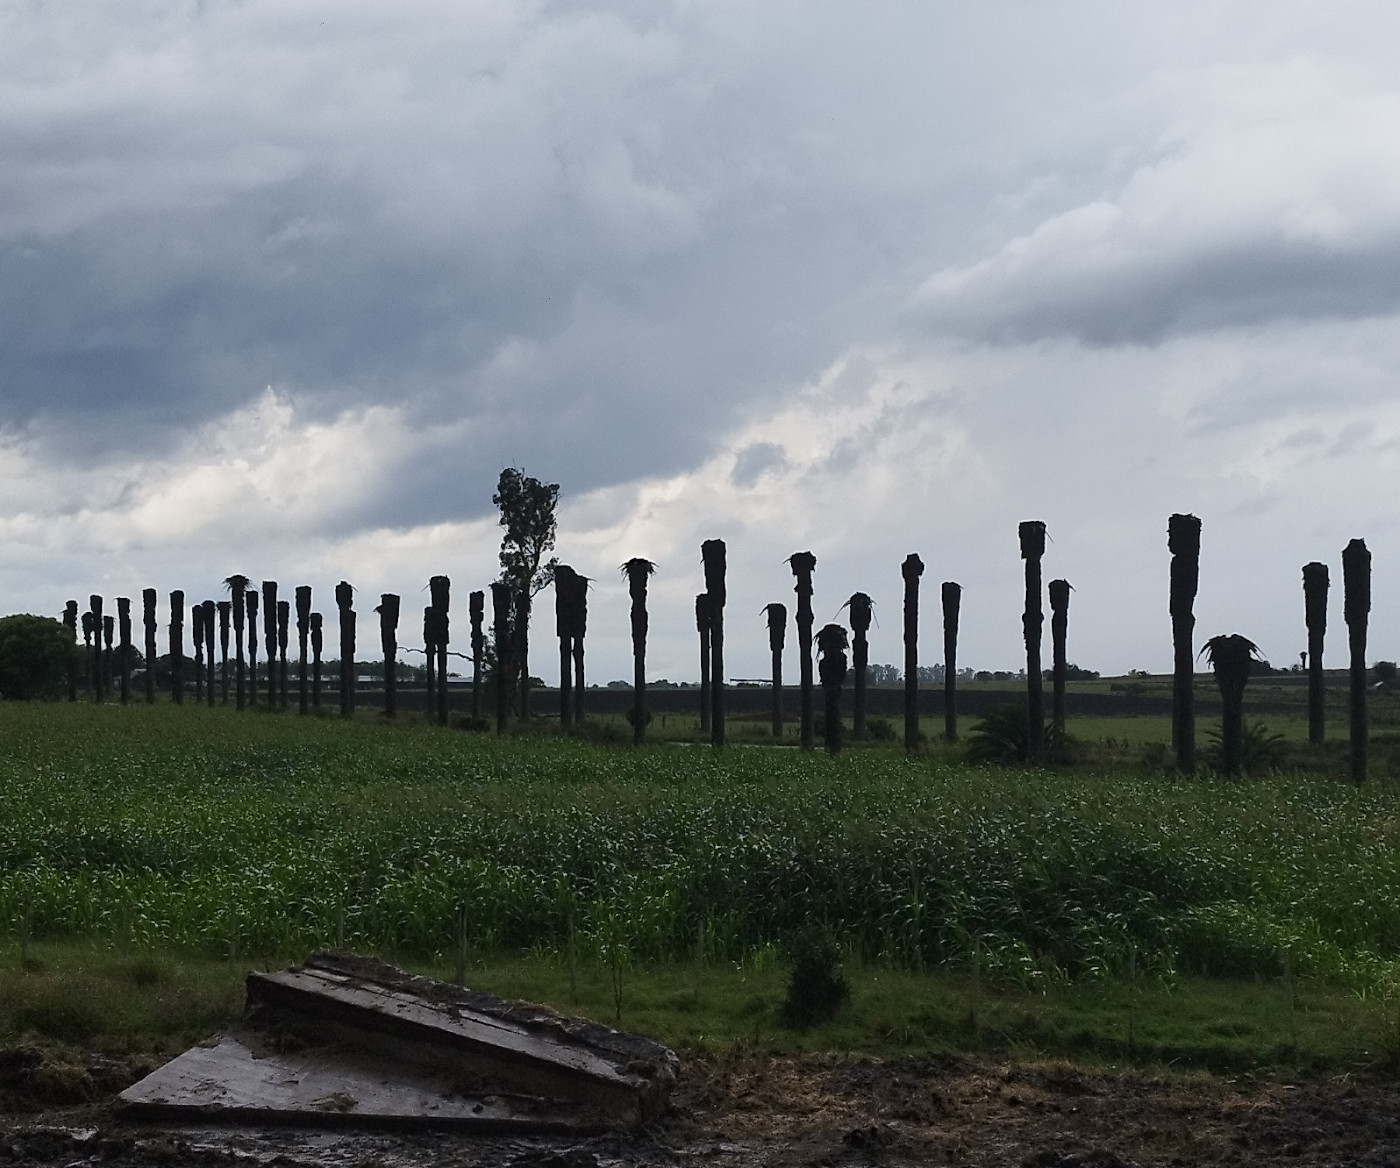
\includegraphics[width=.99\textwidth]{./Figures/palmeras-ruta5.jpg}
    \caption{Palmeras muertas en la ruta 5 de Uruguay.}
    \label{fig:palmeras-ruta5}
  \end{subfigure}
  \caption{Infección y muerte de palmeras por el picudo rojo.}
  \label{fig:infeccion-y-muerte-palmeras}
\end{figure}

Entre los métodos de control fitosanitarios que se utilizan para combatir la plaga se encuentran la endoterapia \citep{intendencia_de_montevideo_acciones_nodate}, el baño, la cirugía \citep{sanchez_cirugiespecializada_nodate} y finalmente la remoción. Sin embargo, estos métodos son costosos y requieren de un monitoreo constante para detectar la presencia del picudo rojo. Para la IM no es solamente una cuestión ecológica sino también económica. En este sentido, el servicio de arbolado realiza un seguimiento de las palmeras afectadas por la plaga. Para ello, se registra su ubicación y estado de salud mediante campañas de detecciones a pie. Este proceso manual requiere de mucho tiempo y recursos humanos, por lo que resulta imprescindible un sistema automatizado que permita detectar la presencia de la plaga en lugares específicos de Montevideo.

Uno de los recursos aún no explotados por la IM para el monitoreo de la plaga es el uso de imágenes aéreas obtenidas mediante drones, disponibles por el servicio de geomática de ésta institución. Estos ortomosaicos, que pueden observarse en la figura \ref{fig:ejemplo-ortomosaico}, permiten obtener información detallada sobre el estado de las palmeras y su entorno.

\begin{figure}[H]
  \centering
  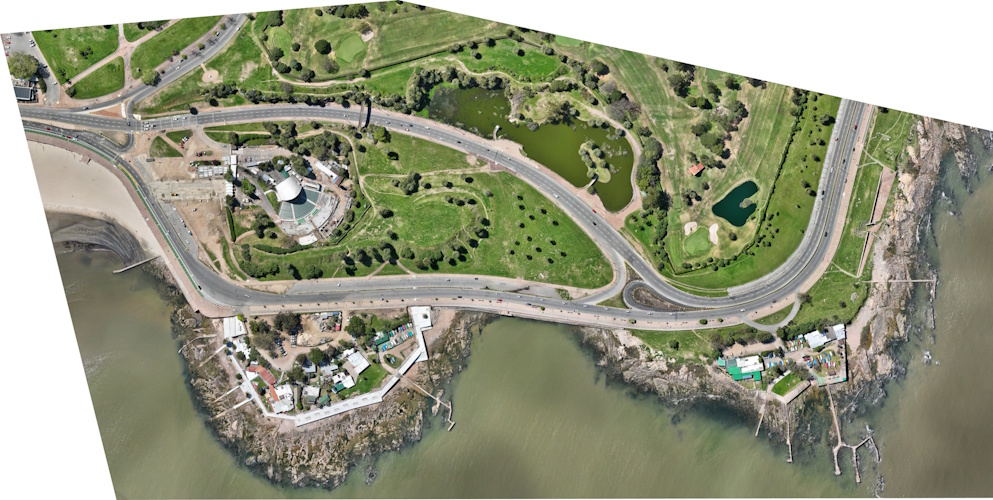
\includegraphics[scale=0.5]{./Figures/ejemplo-ortomosaico.jpg}
  \caption{Ejemplo de ortomosaico \protect\footnotemark.}
  \label{fig:ejemplo-ortomosaico}
\end{figure}

\footnotetext{Imagen tomada del sistema de información geográfica de la IM (SIG): \url{https://sig.montevideo.gub.uy/}}

El análisis de estas imágenes es un proceso complejo que requiere de técnicas avanzadas de procesamiento de imágenes y aprendizaje automático, así como también herramientas que brinden soporte a estas actividades.

%--------------------------------------------------------------------------------------------------------------------------------------------------------------------------------
\section{Estado del arte}
\label{sec:estadoArte}

En los últimos años, el campo de la visión por computadora (VPC) ha experimentado un crecimiento exponencial, impulsado principalmente por los avances en el aprendizaje profundo y las redes neuronales convolucionales (CNN, por su sigla en inglés de \textit{Convolutional Neural Networks}). Estas tecnologías han permitido el desarrollo de soluciones innovadoras para tareas de detección, clasificación y segmentación en imágenes, lo que ha abierto nuevas posibilidades para aplicaciones en diversos ámbitos, tales como la monitorización ambiental y la agricultura de precisión. La detección de plagas mediante imágenes aéreas, en particular la del picudo rojo, ha cobrado relevancia debido al creciente impacto que este insecto tiene en la salud de las palmeras urbanas, principalmente en países del Mediterráneo y en el Medio Oriente \citep{poplin_palm_2014}.
En esta sección se revisan las principales técnicas y enfoques que han marcado el estado del arte en la detección de plagas a partir de imágenes aéreas. Se aborda tanto arquitecturas tradicionales como las más recientes, donde se destacan sus fortalezas, limitaciones y la evolución de sus aplicaciones en escenarios reales.

\subsection{Redes convolucionales}
\label{sec:redesConvolucionales}

La visión por computadora abarca una amplia gama de tareas, tales como la detección de objetos, la segmentación de imágenes, el reconocimiento de patrones y la clasificación de imágenes. Estas tareas suelen abordarse mediante modelos de CNN. Tendencias recientes evidencian avances significativos en el diseño de estas redes para el procesamiento de imágenes. En particular, se ha puesto énfasis en el tratamiento de imágenes de alta resolución capturadas mediante vehículos aéreos no tripulados (UAV, por su sigla en inglés de \textit{Unmanned Aerial Vehicles}), lo que representa un área de aplicación de creciente interés del sector académico y privado \citep{gao_recent_2024} \citep{sutar_convolutional_2025}.

\subsection{Detección del picudo rojo en imágenes aéreas}

La relevancia de la detección de la plaga del picudo rojo a nivel global ha propiciado el surgimiento de diversas líneas de investigación. En este sentido, se han desarrollado enfoques basados en VPC a partir de imágenes aéreas, haciendo especial uso de arquitecturas de CNN tales como YOLO \citep{redmon_you_2016}.

Entre los estudios analizados, la implementación de la detección mediante imágenes aéreas de forma exclusiva representa una metodología relativamente novedosa. En este contexto, en el estudio \textit{Automatic large scale detection of red palm weevil infestation using street view images} \citep{kagan_automatic_2021}, se emplea un enfoque combinado. Inicialmente, se localizan las palmeras a través de una CNN (Faster R-CNN \citep{ren_faster_2016}) aplicada a imágenes aéreas. Posteriormente, utilizando la misma arquitectura, se extrae la corona de la palmera a partir de imágenes capturadas en \textit{street view}, lo que permite clasificar a la planta en función de la presencia o ausencia de infección. Un resumen de este trabajo se presenta en la figura \ref{fig:kagan-automatic-2021-process}.

\begin{figure}[htpb]
  \centering
  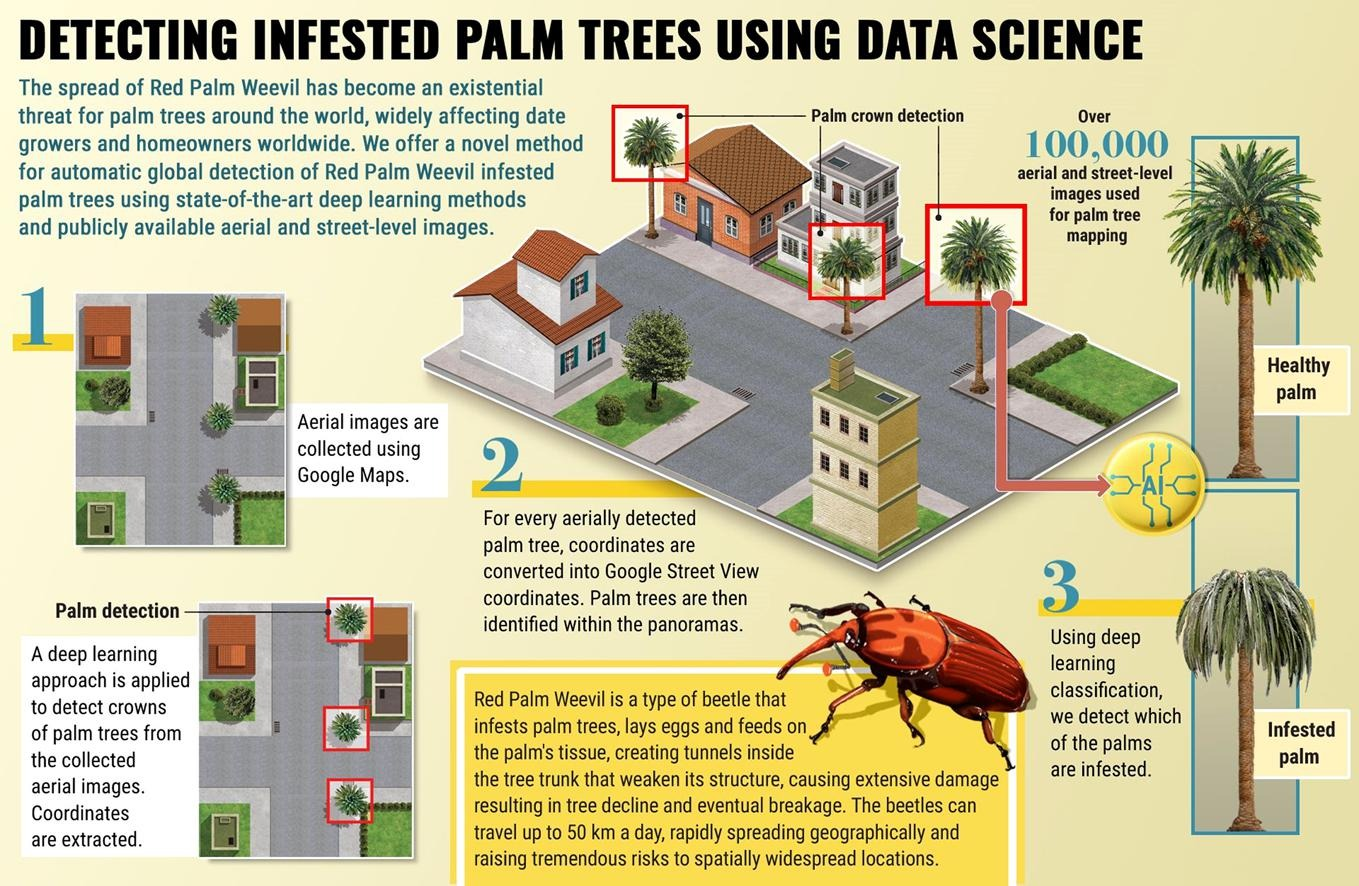
\includegraphics[scale=1.8]{./Figures/kagan_automatic_2021-process.jpg}
  \caption{Proceso de detección realizado por Kagan et al \protect\footnotemark.}
  \label{fig:kagan-automatic-2021-process}
\end{figure}

\footnotetext{Imagen obtenida de: \url{http://arxiv.org/abs/1506.01497}}

Por otro lado, la detección de palmeras sí es ampliamente estudiada en la literatura, siendo un tema recurrente en la investigación de VPC. Se han desarrollado diversos estudios. En \textit{Implementation of slicing aided hyper inference (SAHI) in YOLOv8 to counting oul palm trees using high-resolution aereal imagery data} \citep{zhorif_implementation_2024} se presenta un enfoque que utiliza la arquitectura YOLOv8 para detectar palmeras en imágenes aéreas de alta resolución. Además, utiliza \textit{Slicing Aided Hyper Inference} para mejorar la precisión de la detección. Este enfoque se basa en la idea de dividir las imágenes en regiones más pequeñas y realizar inferencias en cada una de ellas, lo que permite una detección más precisa de los objetos de interés, algo esencial en el caso de objetos pequeños como las palmeras. Para el estudio, se utilizaron imágenes RGB capturadas con un dron Trinity F90+ a 200 metros de altura y una implementación de segmentación (SAHI) de \SI{3000}{}\,\texttimes\,\SI{3000}{\pixel}. Si bien el estudio se centra en la detección de palmeras de aceite, su metodología puede ser adaptada para la detección del picudo rojo. La tabla \ref{tab:papers-deteccion-palmeras} resume los métodos utilizados en la detección de palmeras en diferentes estudios anteriores.

\begin{table}[h]
  \centering
  \caption[comparativa-papers]{Comparación entre diferentes estudios de detección de palmeras\footnotemark.}
  % \begin{adjustbox}{width=\textwidth}
  \begin{tabular}{l c c}
    % \begin{tabular}{{l p{4cm} p{4cm}}}
    \toprule
    \textbf{Autor y año}                                           & \textbf{Método}       & \textbf{Evaluación}               \\
    \midrule
    Mukhles Sir Monea et al, 2022 \citep{muna_development_2023}        & YOLOv3                & 5.76\% (MAPE)                     \\
    Hery Wibowo et al, 2022 \citep{wibowo_large-scale_2022}            & \makecell[c]{YOLOv3,                                      \\YOLOv4, \\YOLOv5m}            & \makecell[c]{97.28\% (v3), \\97.74\% (v4), \\94.94\% (v5m). \\(F1-Score)}              \\
    Adel Ammar et al, 2022 \citep{ammar_deep-learning-based_2021}      & Faster R-CNN          & \makecell[c]{94.99\% (Precision), \\84\% (Recall), \\83\% (AP IoU)}                 \\
    Wardana et al, 2023 \citep{wardana_detection_2023}                 & YOLOv8                & \makecell[c]{98.50\%              \\(Overall Accuracy)}        \\
    Deta Sandya Prasitha et al, 2022 \citep{prasvita_automatic_nodate} & \makecell[c]{YOLOv5s,                                     \\YOLOv5m, \\YOLOv5l, \\YOLOv5x} & \makecell[c]{0.82 (v5s), \\0.84 (v5m), \\0.85 (v5l), \\0.86 (v5x). \\(Average F1-Score)} \\
    Nuwar et al, 2022 \citep{nuwara_modern_2022}                       & YOLOv5                & 0.895 (F1-Score)                  \\
    Junos et al, 2022 \citep{junos_notitle_nodate}                     & YOLOv3n               & \makecell[c]{97.20\% (mAP),       \\0.91 (F1-Score)}                                     \\
    \bottomrule
    \hline
  \end{tabular}
  % \end{adjustbox}
  \label{tab:papers-deteccion-palmeras}
\end{table}

\footnotetext{Tabla obtenida de \textit{Implementation of slicing aided hyper inference (SAHI) in YOLOv8 to counting oul palm trees using high-resolution aereal imagery data} \citep{zhorif_implementation_2024}}

También, se han realizado estudios controlados como en \textit{Red Palm Weevil Detection in Date Palm Using Temporal UAV Imagery} \citep{delalieux_red_2023}, en donde se concluye que la detección del picudo rojo es posible mediante imágenes aéreas en el rango infrarrojo.

%--------------------------------------------------------------------------------------------------------------------------------------------------------------------------------

\section{Objetivos y alcance}
\label{sec:objetivos}

La finalidad principal del presente trabajo consistió en validar una prueba de concepto para la detección tardía del picudo rojo en palmeras de Montevideo, utilizando imágenes aéreas capturadas mediante drones. Con este objetivo, se desarrolló un sistema fundamentado en técnicas de VPC y aprendizaje profundo, que permiten identificar la presencia de la plaga. Para ello, se utilizó la información centralizada en el SIG \citep{intendencia_de_montevideo_sistema_nodate}, complementado con herramientas adicionales que facilitaron la generación del conjunto de datos de entrenamiento.

Adicionalmente, se planteó ante la IM la necesidad de optimizar los procesos de detección de la plaga, con miras a una mejora en la asignación de recursos humanos y económicos. El alcance del trabajo se centró en el desarrollo de una plataforma que permite a los usuarios del sector de áreas verdes de la IM realizar un seguimiento de la expansión de la plaga mediante el monitoreo del estado de salud de las palmeras. En los capítulos siguientes se detalla tanto la descripción de las herramientas utilizadas como el proceso metodológico implementado.